% (c) 2020 Stefan Antonowicz
% Based off of tex found at https://github.com/ludus-leonis/nipajin
% This file is released under Creative Commons Attribution-NonCommercial-ShareAlike 4.0 International License.
% Please do not apply other licenses one-way.

\renewcommand{\yggMechanics}{%
  \mychapter{Mechanics}{core-mechanics}
}

\renewcommand{\yggMechanicsText}{%


\mysection{Rolls}{rolls}

There are 3 types of "special" die rolls in ToY

\mytable{X c}{
  \thead{Roll} & \thead{Symbol} \\
}{
    Roll 20 & \RO \\
    Roll to Beat & \RB \\
    Roll to Succeed & \RS \\
}

Rolls are distinct from one another i.e. powers and abilities that affect \RO (like a Knave's Luck Die) cannot affect \RB or \RS.  

Making an \RO, \RB, or \RS attempt is a \mybold{try}

\mysubsection{Roll Twenty}{rolls-roll-twenty}
In a \RO try you have to roll a 20 or better with a combination of dice and modifiers. A 19 misses, a 20 succeeds. 

\mysubsection{Roll to Beat}{rolls-roll-to-beat}
In a \RB try you roll a single die plus modifiers and try to beat 1 or more other \RB rolls.  The type of die will be defined with the \RB



\example {%
  An orc trys to push a barbarian off a ledge.  Both the orc and the barbarian try a \RB : \VIG test, highest roll wins \\ ~\\ A sorcerer casts Battering Beam at a kobold.  The kobold fails its Save and must try a \RB : \VIG vs. the sorcerer's \INT \\ ~\\ Two Allies rush toward an idol teetering on the brink of a chasm.  They each try a \RB : \MD+\DEX test to see who gets there first
}



When Monsters try a \RB, they add their \HD as a modifier to their test i.e. a 6\HD Monster adds +6 to their \RB roll.  When Allies roll a \RB, they add their level as a modifier to their test \mybold{if} they are rolling their \mylink{Primary Stat}{primary-stat}.

Ties go to the Allies.  If there's a tie between Allies, roll a d6 and add its result to your \RB until there's a winner.

\cbreak\bump

\mysubsection{Roll to Succeed}{rolls-roll-to-succeed}
To roll to succeed, you must roll a die without rolling a Failure (a natural 1 or 2).  \RS rolls cannot be modified (though they can sometimes be changed).  

\mysubsection{Failure}{rolls-failure}
A Failure occurs when you roll a \myital{natural} 1 or 2 on a \RS (\myital{natural} means that's what's on the face of the die). Failure has different effects depending on the type of die you might be rolling.  Details of what happens if you fail will be in the description of the roll.

\begin{center}
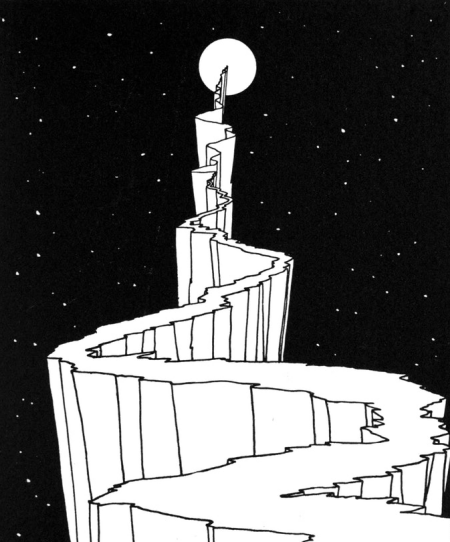
\includegraphics[scale=.25]{Moonscape}
\end{center}


\newpage

\mysection{Dice}{dice}
The ToY rules use 10 different dice: d24, d20, d16, d12, d10, d8, d6, d4, d3, and d2 (a coin flip).   If you were to dump out all the dice in your Crown Royal bag and put them in order from lowest to highest (d2, d3, d4, etc), you'd have a Dice Chain

\mysubsection{Dice Chains}{dice-dice-chains}
The ToY dice chain is:
~\\

\example {%
  \mybold{d2 \DubArrw d3 \DubArrw d4 \DubArrw d6 \DubArrw d8 \DubArrw d10 \DubArrw d12 \DubArrw ... \\ ... d16 \DubArrw d20 \DubArrw d24}
}
\mylist {%
  \item When you see \DCUP , move 1 up the dice chain (so from a d6 to a d8).
  \item When you see \DCDOWN , move 1 down the dice chain (so from a d6 to a d4).  
}

Dice can't go higher than d24 or lower than d2.  If a die is \mybold{exhausted}  that means it is lost (set to 0).

\mysubsection{Static Dice}{dice-static-dice}
\example{%
  \STATIC \\
  \mybold{The base die used in \RO and \RB tries.}
}

Static dice are dice used in \RO and \RB tries; they are often combined together with other modifiers to get to a 20 or better.

\cbreak\bump


\mysubsection{Usage Dice}{dice-usage-dice}
\example{% 
 \UD \\
  \mybold{A die used to \RS or modify \RO tries. It moves \DCDOWN on a Failure}
}

\ed{To the best of my knowledge, the Usage Die is a mechanic invented by David Black.}

When you roll a \UD, the die moves \DCDOWN on a Failure.  If your \UD is a d2, it's automatically exhausted after you roll.  

All \UD have a maximum (\MAX) and current value.  For example, your \UD for your Armor might be a d8 \MAX but you've taken a few hits and now it's a d6 (current).  Unless specified, a \DCDOWN or \DCUP refers to the "current" value.  i.e.  "your Presence moves \DCDOWN" vs. "your \MAX Presence moves \DCDOWN"

\mysubsection{Pool Dice}{dice-pool-dice}
\example{%
  \POOL \\
  \mybold{A die used to \RS.  It is exhausted on a Failure} 
}

Pool dice are like \UD, except the die is immediately exhausted when you roll a Failure (it doesn't move \DCDOWN like a \UD does).  

\newpage

\mysection{Tangible Stats}{tangible-stats}

Tangible Stats are the physical, definable aspects of your character.  Tangible Stats are \STATIC and don't go up or down unless something really bad happens.

Each \mylink{Mortal Trope}{mortals} has a \myanchor{Primary Stat}{primary-stat} listed below.

\mysubsection{Vigor}{tangible-stats-vigor}

How strong you are, how much pain and hardship you can endure, your physical essence.  In \mylink{Combat}{combat}, \VIG is used when \mylink{Fighting}{combat-fighting} with Hard weapons. \VIG is the Primary Stat for \mylink{Sellswords}{trope-sellsword}. 

\mysubsection{Dexterity}{tangible-stats-dexterity}

How adroit you are, your hand-eye coordination, your speed.  In \mylink{Combat}{combat}, \DEX is used when \mylink{Fighting}{combat-fighting} with Fast weapons and \mylink{Guarding}{combat-guarding} against attacks. \DEX is the Primary Stat for \mylink{Knaves}{trope-knave}.  


\mysubsection{Intellect}{tangible-stats-intellect}

How smart you are, how observant you are, how easy it is for you to learn and remember things. In \mylink{Combat}{combat}, \INT is combined with your Move Die to determine \mylink{Init}{combat-init} (when you get to take your turn in Combat). \INT is the Primary Stat of \mylink{Philosophers}{trope-philosopher}.  


\mysubsection{Focus}{tangible-stats-focus}

How well you can concentrate, how patient you are, your will to live, your ability to observe and control magical energies.  In \mylink{Combat}{combat}, \FOC is rolled for \mylink{Crits and Fumbles}{combat-crits-and-fumbles} and when you are \mylink{Dying}{combat-dying}.  \FOC is the Primary Stat of \mylink{Mystics}{trope-mystic}

\cbreak


\mysection{Intangible Stats }{intangible-stats}


Intangible Stats are the nonphysical, abstract aspects of your character. Intangible Stats are \UD and their die will decrease with use.  You can use your Intangible Stats to modify any \RO or \RB try using its \myital{corresponding} Tangible Stat (see below).

Each \mylink{Unseelie Species}{unseelie} has a \myanchor{Primary Stat}{primary-stat} listed below.


\mysubsection{Presence}{intangible-stats-presence}

Confidence, attractiveness, leadership, and intimidation. The Arbiter might ask you if you'd like to roll your Presence \UD if you're trying to sweet talk someone, keep a group of peons from breaking morale, or scaring a couple of kobolds into telling you what you want to know. 

You can roll your Presence die and add its result to any \RO or \RB try you're making that involves \VIG.  If your Presence is exhausted, your confidence ebbs: you are unable to heal Grit until you gain a Presence \UD back.

Presence is the Primary Stat for \mylink{Pooka}{species-pooka}.


\mysubsection{Talent}{intangible-stats-talent}

It always seems like you're in the right place at the right time, or that you have the favor of the Gods. The Arbiter might ask you if you'd like to roll your Talent \UD if you're trying to see if something works by pure random luck ("I randomly press buttons on the console and hope something good happens"; "I close my eyes and try to jump off the roof into the hay cart").  

You can roll your Talent die and add its result to any \RO or \RB try you're making that involves \DEX.  If your Talent is exhausted, your luck has run out: you automatically take a 1 in any \mylink{Luck Contests}{other-stuff-luck-contests} until you gain a Talent \UD back.

Talent is the Primary Stat for \mylink{Night Children}{species-night-child}

\newpage

\mysubsection{Awareness}{intangible-stats-awareness}

Your idle perception, your "sixth sense".   The Arbiter will ask you to roll your Awareness to  notice something that you might not be actively looking for (you can say no!).  

You can roll your Awareness die and add its result to any \RO or \RB try you're making that involves \INT.  If your Awareness is exhausted, you are mentally fogged: you always lose Init until you gain an Awareness \UD back.

Awareness is the Primary Stat for \mylink{Spriggan}{species-spriggan}

\cbreak

\mysubsection{Sanity}{intangible-stats-sanity}

How lucid you are, and how likely you are to keep your cool.  The Arbiter might tell you to make a Sanity roll when you see something particularly heinous (you don't get to say no on this one).  

You can roll your Sanity \UD and add its result to any \RO or \RB try you're making that involves \FOC.  If you ever Fail a Sanity roll (roll a 1 or a 2), you must roll on \mylink{Terrifying Tables}{misc-terrifying-tables} (the Arbiter will determine which table to roll on). If your Sanity is exhausted, you immediately gain the Madness \mylink{Shot Nerves}{madness-shot-nerves} in addition to any other Madnesses until you gain a Sanity \UD back.

Sanity is the Primary Stat for \mylink{Murks}{species-murk}

\end{multicols}
\begin{center}
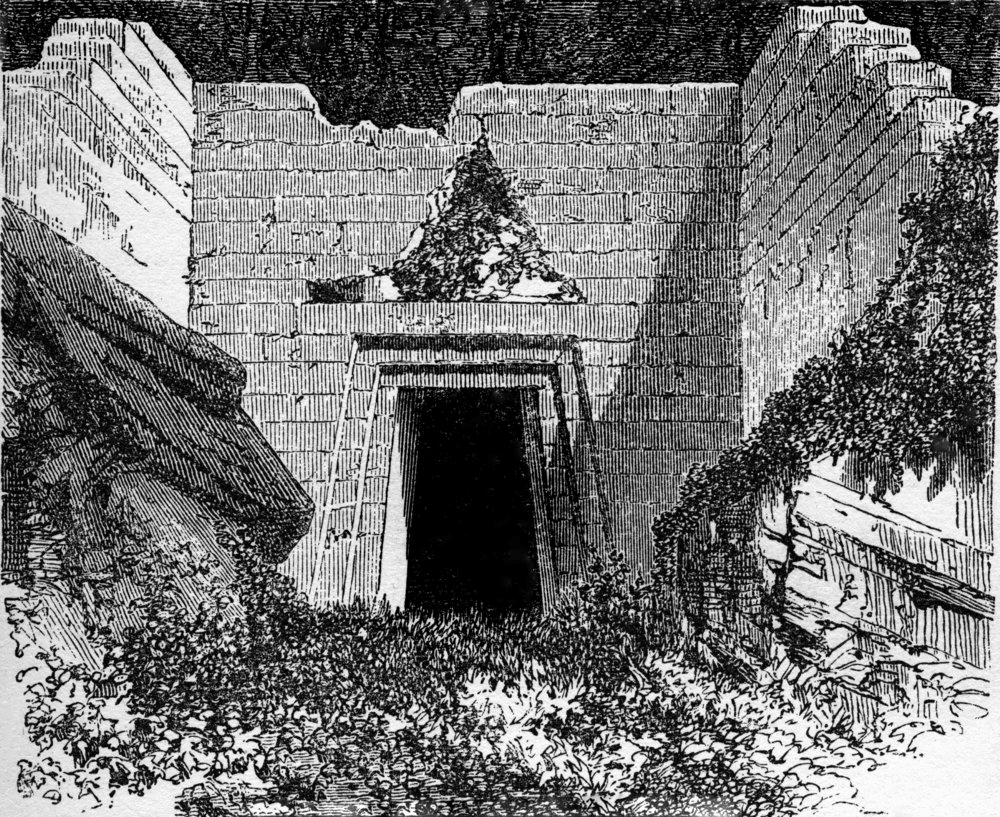
\includegraphics[scale=.4]{Doorway}
\end{center}


\newpage

\begin{multicols*}{2}


\mysection{Time}{time}

Time is divided into abstracts:  Moments, Minutes, Hours, Days, Weeks, Years, etc.  No specific amount of time is specified i.e. "that will take Minutes to do" or "you'll need to rest for Hours"

\mysubsection{Combat}{time-combat}

Combat is divided into Moments and takes Minutes to complete.  You can take 1 or 2 Actions every Moment, depending on your \mylink{Init}{combat-init}.

\mybold{\myhighlight{Top Of / Bottom Of ...}{time-top-bottom}}

Effects that happen at the top of the Moment occur immediately before \mybold{you personally} take your first Action, but after you've rolled \mylink{Init}{combat-init}.

Effects that happen at the bottom of the Moment occur immediately after \mybold{everyone} (including Monsters) has taken all their Actions, \myital{before} \mylink{Init}{combat-init} is rolled.


\mybold{\myhighlight{Markovian}{time-markovian}}

Some spells or effects have a "Markovian" duration.  Markovian effects start immediately but have a random duration over the course of Moments. Markovian durations have a duration die attached to them i.e "d4 Markovian".

At the bottom of a Moment, \RS using the effect's duration die.  If you roll a Failure (a 1 or a 2) for the effect, it immediately ends.  Otherwise, the duration die moves \DCDOWN. 

For example, if you were struck by a Ghast and paralyzed for d4 Markovian, you would roll a d4 at the bottom of the Moment for the effect.  If you rolled a 1 or a 2, the paralysis effect would end.  If you rolled a 3 or a 4, the die would move to a d3.

\mysubsection{Session}{time-session}

When you sit down to play, this begins a "session".  When the game stops and everyone goes home, that ends the session.  

\cbreak\bump

\mysubsection{Adventure}{time-adventure}

Determined by the Arbiter, see the section on \mylink{Adventures}{advancement-adventuring}.

\mysubsection{Resting}{time-resting}

Using time to rest is divided into 3 groups:

\mynumlist {
    \item \mybold{Taking a Breather}:  \\~  Takes Minutes.  More details found in \mylink{Combat}{combat-resting-breather}
    \item \mybold{Taking a Bivouac}:  \\~ Takes Hours.  More details found in \mylink{Combat}{combat-resting-bivouac}
    \item \mybold{Taking a Vacation}:  \\~ Takes Days or Weeks.  More details found in \mylink{Civilization}{civilization-vacation}
}



\mysection{Distance}{distance}

\mysubsection{Combat}{distance-combat}

Like Time, Distance is broken into abstract lengths: \mybold{Close}, \mybold{Nearby}, \mybold{Far-Away}, and \mybold{Distant}.  \MAX Combat distance is 100 meters

\mytable{X c}{
  \thead{} & \thead{} \\
}{
    Close & \Tilde 1m \\
    Nearby & \Tilde 10m \\
    Far Away & \Tilde 50m \\
    Distant & \Tilde 100m \\
}


\mysubsection{Non-Combat}{distance-non-combat}

Non Combat distances are covered in the Arbiter's section on \mylink{Travel}{arbiter-travel}


\cbreak


\mysection{Other Stuff}{other-stuff}


\mysubsection{Terror Horror and Madness}{other-stuff-terror-horror-madness}

Bearing witness to horrible or terrible things can prompt a roll of your Sanity \UD.  If you roll a Failure, you must roll on the \mylink{Terrifying Tables}{misc-terrifying-tables} (the Arbiter will determine which table to roll on). 

Examples that might prompt a Sanity roll:  witnessing a member of the party getting killed; a horrifying creature you've never seen before; a situation that shakes your beliefs; or not \mylink{Dying}{combat-dying}

\cbreak\bump

\mysubsection{Luck Contests}{other-stuff-luck-contests}

The Arbiter may call for a Luck Contest if she is trying to figure out what random bad thing is going to happen to someone ("the ogre turns his attention towards one of you"; "one of you gets hit with 2 effects, not just one", etc. )

You can choose to roll \mybold{any} \mylink{Intangible Stat}{intangible-stats} \UD you choose.  Instead of rolling the \UD, you can opt to "take a one" (meaning your roll is an automatic 1).  The person with the lowest roll is the victim. If there's a tie for last (including if multiple people decide to "take a one"), the Arbiter chooses the adventurer with the lowest \MAX Talent.  If there is still a tie, the Arbiter gets to pick (roll randomly or do whatever feels right).

} %end
